\documentclass{standalone}

\usepackage[english]{babel}
\usepackage[linesnumbered, ruled, vlined]{algorithm2e}

\usepackage{graphics}

\usepackage{caption}
\usepackage{subcaption}

% to create listings

\usepackage{listings, lstautogobble}
\lstset{
  autogobble=true,
  frame=single,
}

\lstdefinelanguage{coq}[Objective]{Caml}{
  morekeywords={Structure, Definition, Inductive, list, return},
  sensitive=true
}

% to define font size

\usepackage{ulem}
\usepackage{moresize}
\usepackage{anyfontsize}

% to use tikz and its libraries

\usepackage{tikz-timing}
\usepackage{tikz}

\usetikzlibrary{backgrounds}
\usetikzlibrary{positioning, calc, arrows, shapes, automata, petri, patterns}

% to use tikzmark, to place and refer to marks outside the current figure

\tikzset{every picture/.style={remember picture}}

% styles for transitions

\tikzset{transition/.append style={fill=black!20, thick}}
\tikzset{transition/.append style={fill=black!20, thick}}

% styles for test and inhib arcs.

\tikzstyle{test}=[pre, *-]
\tikzstyle{inhib}=[pre, o-]

% to use colors

\usepackage{xcolor}

%%%%%%%%%%%%%%%%%%%%%%%%%%%%%%%%%%%%%%%%%%%%%%%%%%
%                  BEGIN DOCUMENT                %
%%%%%%%%%%%%%%%%%%%%%%%%%%%%%%%%%%%%%%%%%%%%%%%%%%

\begin{document}

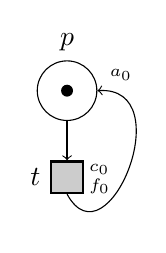
\begin{tikzpicture}

  % \draw[step=5pt] (-.5,-1.7) grid (.9,.8);
  \clip (-.5,-1.7) rectangle (.9,.8);
  
  \node[place, tokens=1]  (p0) [label={above:$p$}] {};
  \node at ($(p0.east)+(.3,.2)$) {\ssmall $a_0$};
  
  \node[transition, anchor=north] (t0) at ($(p0.south)-(0,.5)$) [label={left:$t$}] {};
  \node at ($(t0.east)+(.2,0)$) {
    \ssmall
    \begin{tabular}{@{}l@{}}
      $c_0$ \\
      $f_0$ \\
    \end{tabular}
  };

  \draw ($(p0.south)$) edge[->] ($(t0.north)$);
  \draw ($(t0.south)$) edge[->, bend right, out=-135, in=-70, looseness=2] ($(p0.east)$);

\end{tikzpicture}

\end{document}

%%% Local Variables:
%%% mode: latex
%%% TeX-master: t
%%% End:
